\newline
\subsection{Diagramma delle Attività}
Sono utili per descrivere delle \textcolor{cyan}{attività} relative a un qualsiasi \emph{oggetto} o \emph{classe}, ovvero un insieme di azioni che possono essere \emph{sequenziali},
\emph{condizionali}, \emph{concorrenti} e \emph{iterative}.

Si usano sia nella fase di \emph{analisi} per modellare un processo o un caso d'uso,
ma anche per descrivere l'\emph{operazione} di una classe o per modellare un algoritmo in
fase di \emph{testing}.

Il contenuto di un'attività è un \emph{grafo diretto} in cui i \textcolor{cyan}{nodi} sono
le \emph{azioni} o i \emph{nodi di controllo}, mentre gli \textcolor{cyan}{archi} sono i possibili
percorsi percorribili per l'attività.

\begin{figure}[h]
    \centering
    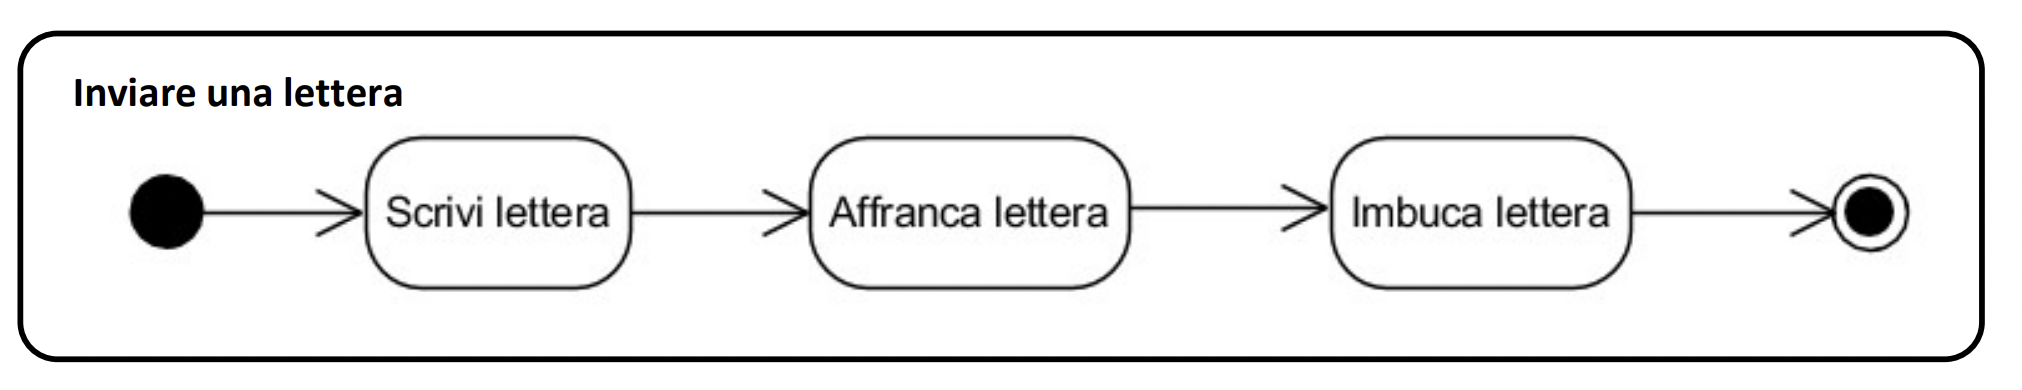
\includegraphics[scale=0.34]{img/azione.png}
\end{figure}

\paragraph{\textcolor{cyan}{Azioni}} È importante sottolineare che le azioni devono essere
\textbf{\textcolor{cyan}{atomiche}}, cioè \underline{non} interrompibili.
Inoltre per ogni azione ci può essere solo una freccia entrante e una uscente.
Quando un'azione è giunta al termina avviene una transazione automatica chiamata
\textbf{\textcolor{cyan}{token}} che porta all'azione successiva.

\begin{figure}[h]
    \centering
    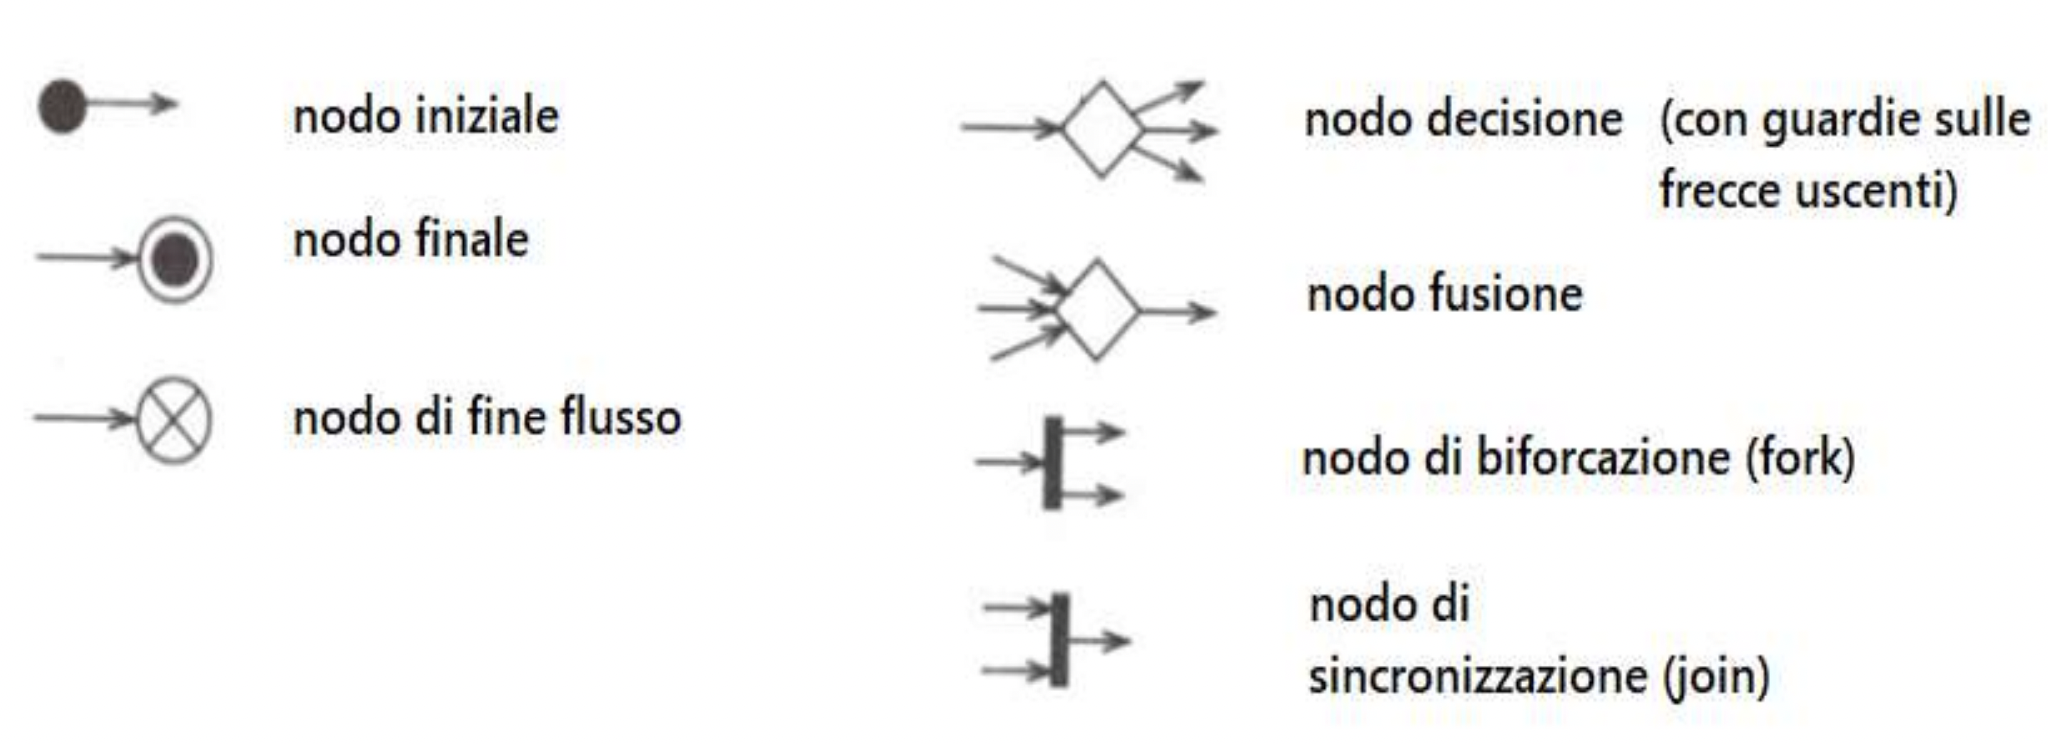
\includegraphics[scale=0.30]{img/nodidecisione.png}
    \caption{Nodi di Controllo}
\end{figure}

\paragraph{\textcolor{cyan}{Nodi di Decisione}} Un nodo di decisione deve poter coprire tutti i casi
possibili, in modo che il \emph{\textcolor{cyan}{token}} non possa bloccarsi. Opzionalmente le \emph{guardie}
possono essere \emph{\textcolor{cyan}{mutualmente esclusive}}.
Inoltre, dato un \emph{nodo decisione} non è obbligatoria la presenza di un \emph{nodo fusione}.

Le \emph{guardie} si scrivono sempre tra parentesi \verb|[]|.

\paragraph{\textcolor{cyan}{Fork \& Join}} La \emph{fork} moltiplica i token, producendone
uno per ogni uscita. La \emph{join} invece attende un token per ogni freccia entrante e, quando li consuma tutti, ne esce
solo uno. Come per i nodo di decisione non è necessaria una \emph{join} per ogni \emph{fork}.

\paragraph{\textcolor{cyan}{Nodo di Fine Attività}} Quando un qualsiasi token raggiunge questo nodo
tutta l'attività termina. Solo su questi nodi, e su quelli di \emph{fine flusso}, possono essere presenti più
archi entranti; ciò sta a significare che il primo token che arriva termina l'attività.

\paragraph{\textcolor{cyan}{Nodo di Fine Flusso}} Questo tipo di nodo non termina l'attività, ma consuma il token.

\subsubsection{Segnali \& Eventi}

\begin{itemize}
    \item Accettazione di un evento esterno.
        \begin{figure}[h]
            \centering
            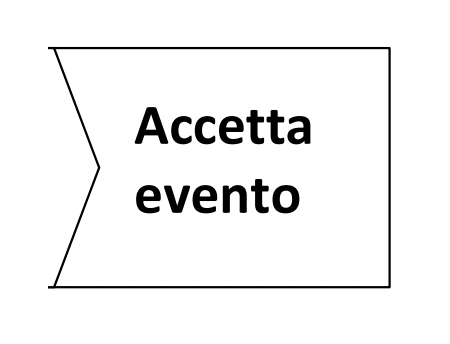
\includegraphics[scale=0.30]{img/accettaevento.png}
        \end{figure}
    \item Invio di un segnale. L'invio di segnali è \textcolor{cyan}{\underline{asincrono}}, cioè non blocca l'attività.
        \begin{figure}[h]
            \centering
            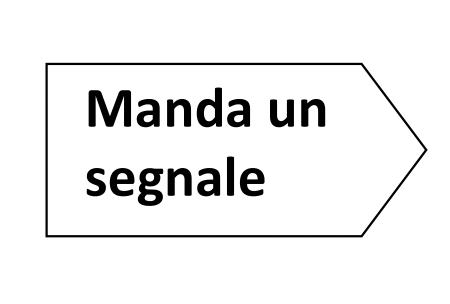
\includegraphics[scale=0.30]{img/mandasegnale.png}
        \end{figure}    
    \item Accettazione di un evento temporale.
        \begin{figure}[H]
            \centering
            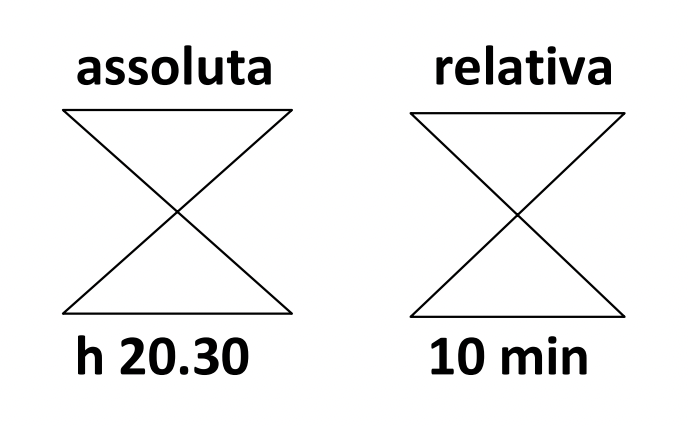
\includegraphics[scale=0.30]{img/tempo.png}
        \end{figure}
\end{itemize}

Per gli eventi \textcolor{cyan}{esterni} e \textcolor{cyan}{temporali}, gli archi entranti non sono
necessari, quindi in questo caso quando si verifica quel determinato evento viene generato un token.
Se invece gli archi entranti sono presenti, quando arriva il token questo attende che l'evento esterno si verifichi.

A differenza delle \textcolor{cyan}{azioni} che si usano quando le attività sono effettuate
dalle entità di cui si sta descrivendo il comportamento, mentre i \textcolor{cyan}{segnali} e gli
\textcolor{cyan}{eventi} si usano quando si comunica con un'entità esterna.

\subsubsection{Sotto-Attività}

Un diagramma può contenere il riferimento a delle attività secondarie, rappresentate
come un'azione ma con in più il simbolo di un "rastrello".

\begin{figure}[h]
    \centering
    \includegraphics[scale=0.45]{img/sottoattività.png}
\end{figure}

\subsubsection{Partizioni}

Le \textbf{\textcolor{cyan}{partizioni}} permettono di dividere le azioni, assegnandole
all'entità che ne è responsabile.